\documentclass[]{article}

\usepackage[backend=bibtex,style=numeric,sorting=none]{biblatex}
\usepackage[hidelinks]{hyperref}
\usepackage{geometry}
\usepackage{graphicx}
\usepackage{subfig}
\usepackage{float}
\usepackage{multicol}

\geometry{
    a4paper,
    left=3.18cm,
    right=3.18cm,
    top=2.54cm,
    bottom=2.54cm
}

\addbibresource{cite.bib}

%opening
\title{\textbf{CS583 Course Project Report: Kannada MNIST}}
\author{Chang Lu}

\setlength{\parskip}{0.6em}

\begin{document}

\maketitle

\section{Summary}
We participate an active competition called \textit{\textbf{Kannada MNIST}}. The main task of this competition is classifying Kannada digits from 0 to 9. Kannada is a language spoken predominantly by people of Karnataka in southwestern India. The language has roughly 45 million native speakers and is written using the Kannada script~\cite{wiki:Kannada}.

The final model we choose is a traditional Convolutional Neural Network, which takes $28 \times 28 \times 1$ images as the input and outputs the class labels of each image. We implement the convolutional neural network using Keras and run the code on a PC with one Intel i9 CPU, 64GB memory and a NVIDIA GeForce RTX 2080Ti GPU. The performance is evaluated on the classification accuracy.

Up to November 30, 2019, we get a 0.98940 score in the public leader board, and the rank is 65 out of 947 teams. As for the private leader board, the result will not be available until December 17, 2019.

\section{Problem Description}
\paragraph{Problem}
This competition Kannada MNIST~\footnote{\url{https://www.kaggle.com/c/Kannada-MNIST/}} aims to classify 10 handwritten Kannada digits based on gray images. \figurename{~\ref{fig:kdigit}} shows the shape of Kannada digit numbers from 0 to 9.
\begin{figure}[H]
    \centering
    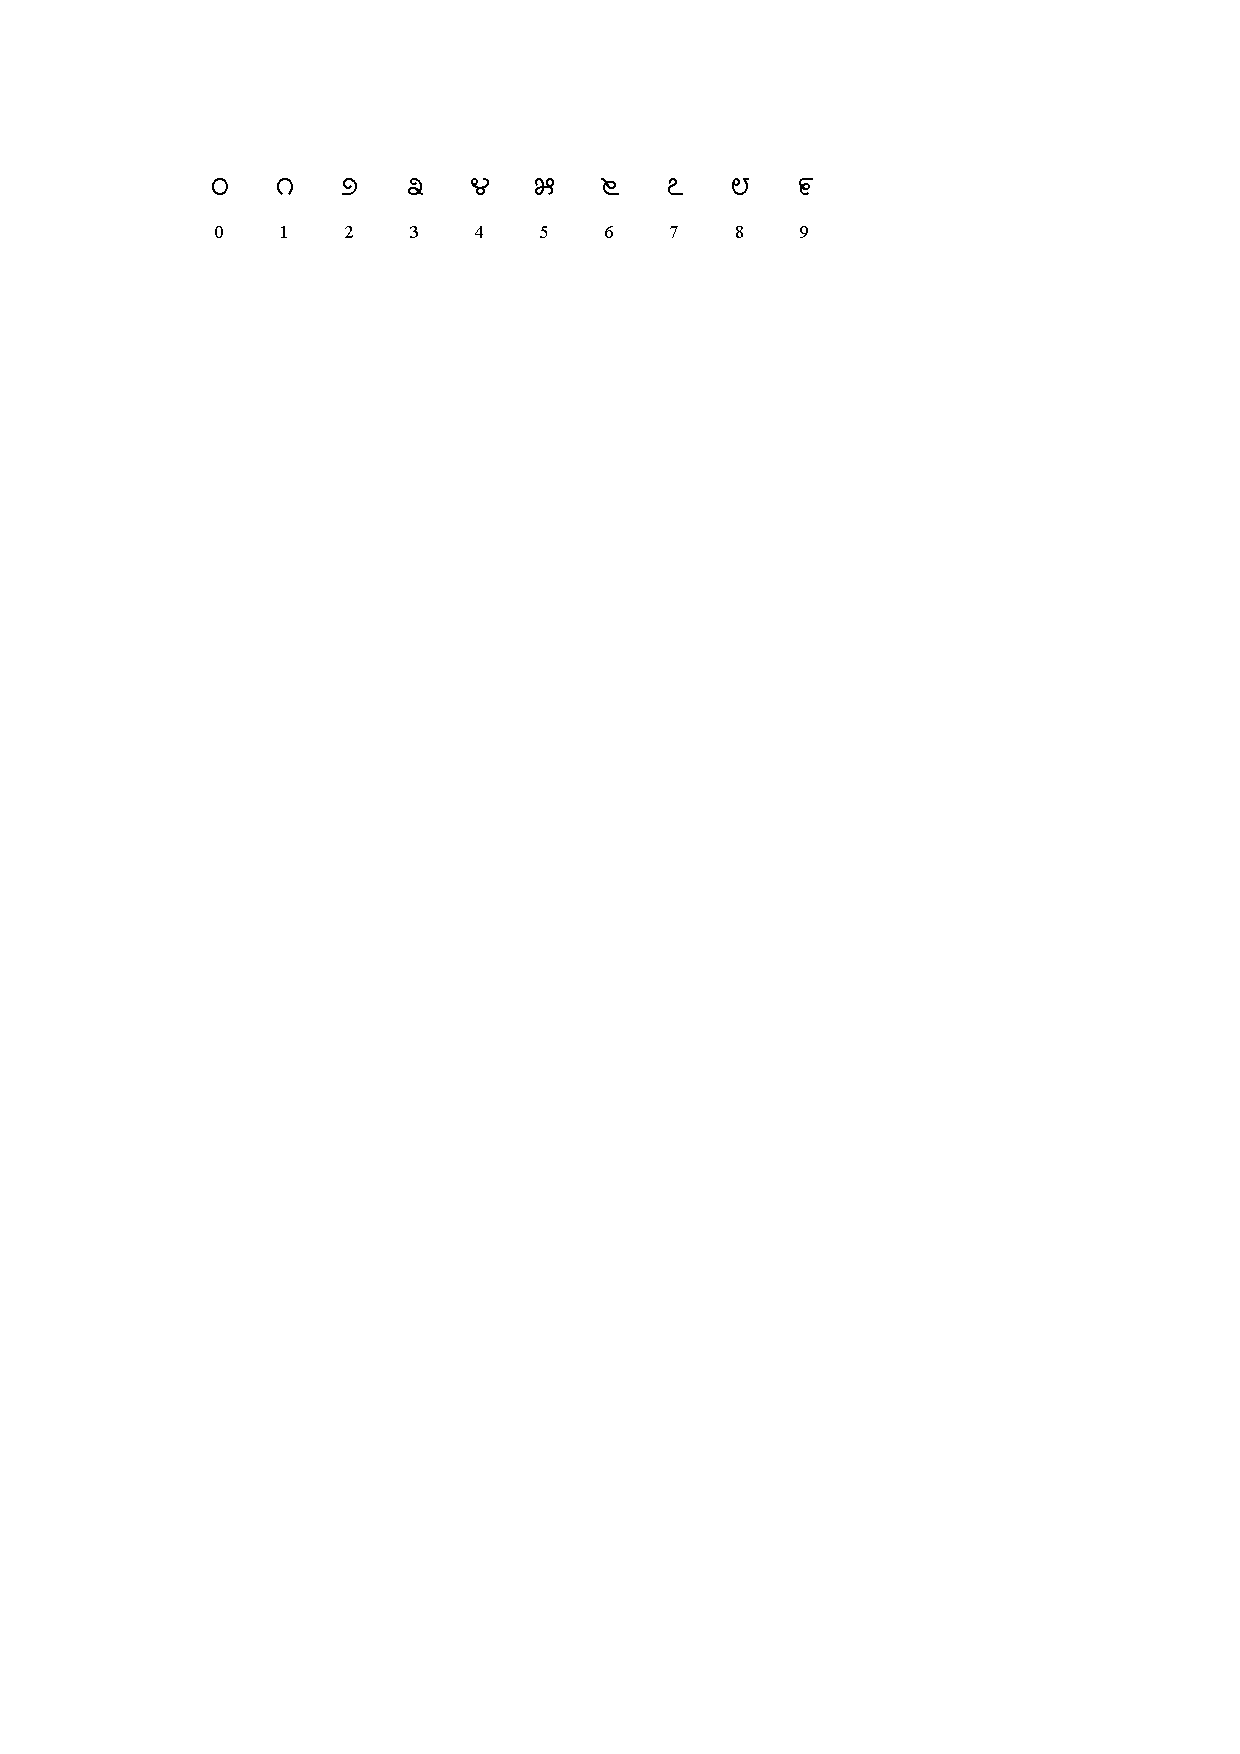
\includegraphics[]{figs/kdigits}
    \caption{Kannada digits from 0 to 9}
    \label{fig:kdigit}
\end{figure}

\paragraph{Data}
The data are $28 \times 28 \times 1$ images and the raw data are stored in CSV files. In the CSV files, one line is an image of which each pixel is a 0 or 1 value in the CSV cell. The number of training samples is $n = 60000$, and the number of testing samples is $10000$. Definitely, the testing samples are hidden from us. The number of class is 10, and the training and testing samples are uniformly distributed across the 10 classes~\cite{prabhu2019kannada}.

\paragraph{Challenges}
This problem is similar to the original MNIST multi-classification task~\cite{lecun:mnist}, but uses Kannada numbers as the input, which could be more confusing in some labels. For example, 0, 1 and 8 are similar. 2 and 3 are also similar to each other.

\section{Solution}
\paragraph{Model}
The model we finally choose is a traditional CNN, which contains 5 blocks. The first 3 blocks consists of 3 convolutional layers, 1 pooling layer and 1 dropout layer. The kernel sizes of convolutional layers in each block are 32, 64 and 128 respectively. The fourth block contains 1 convolutional layers with kernel size of 256, 1 pooling layer and a dropout layer. The final block contains 3 fully-connected layers and the last one is the output layer. The model are demonstrated in \figurename{~\ref{fig:modelcnn}}.
\begin{figure}[H]
    \centering
    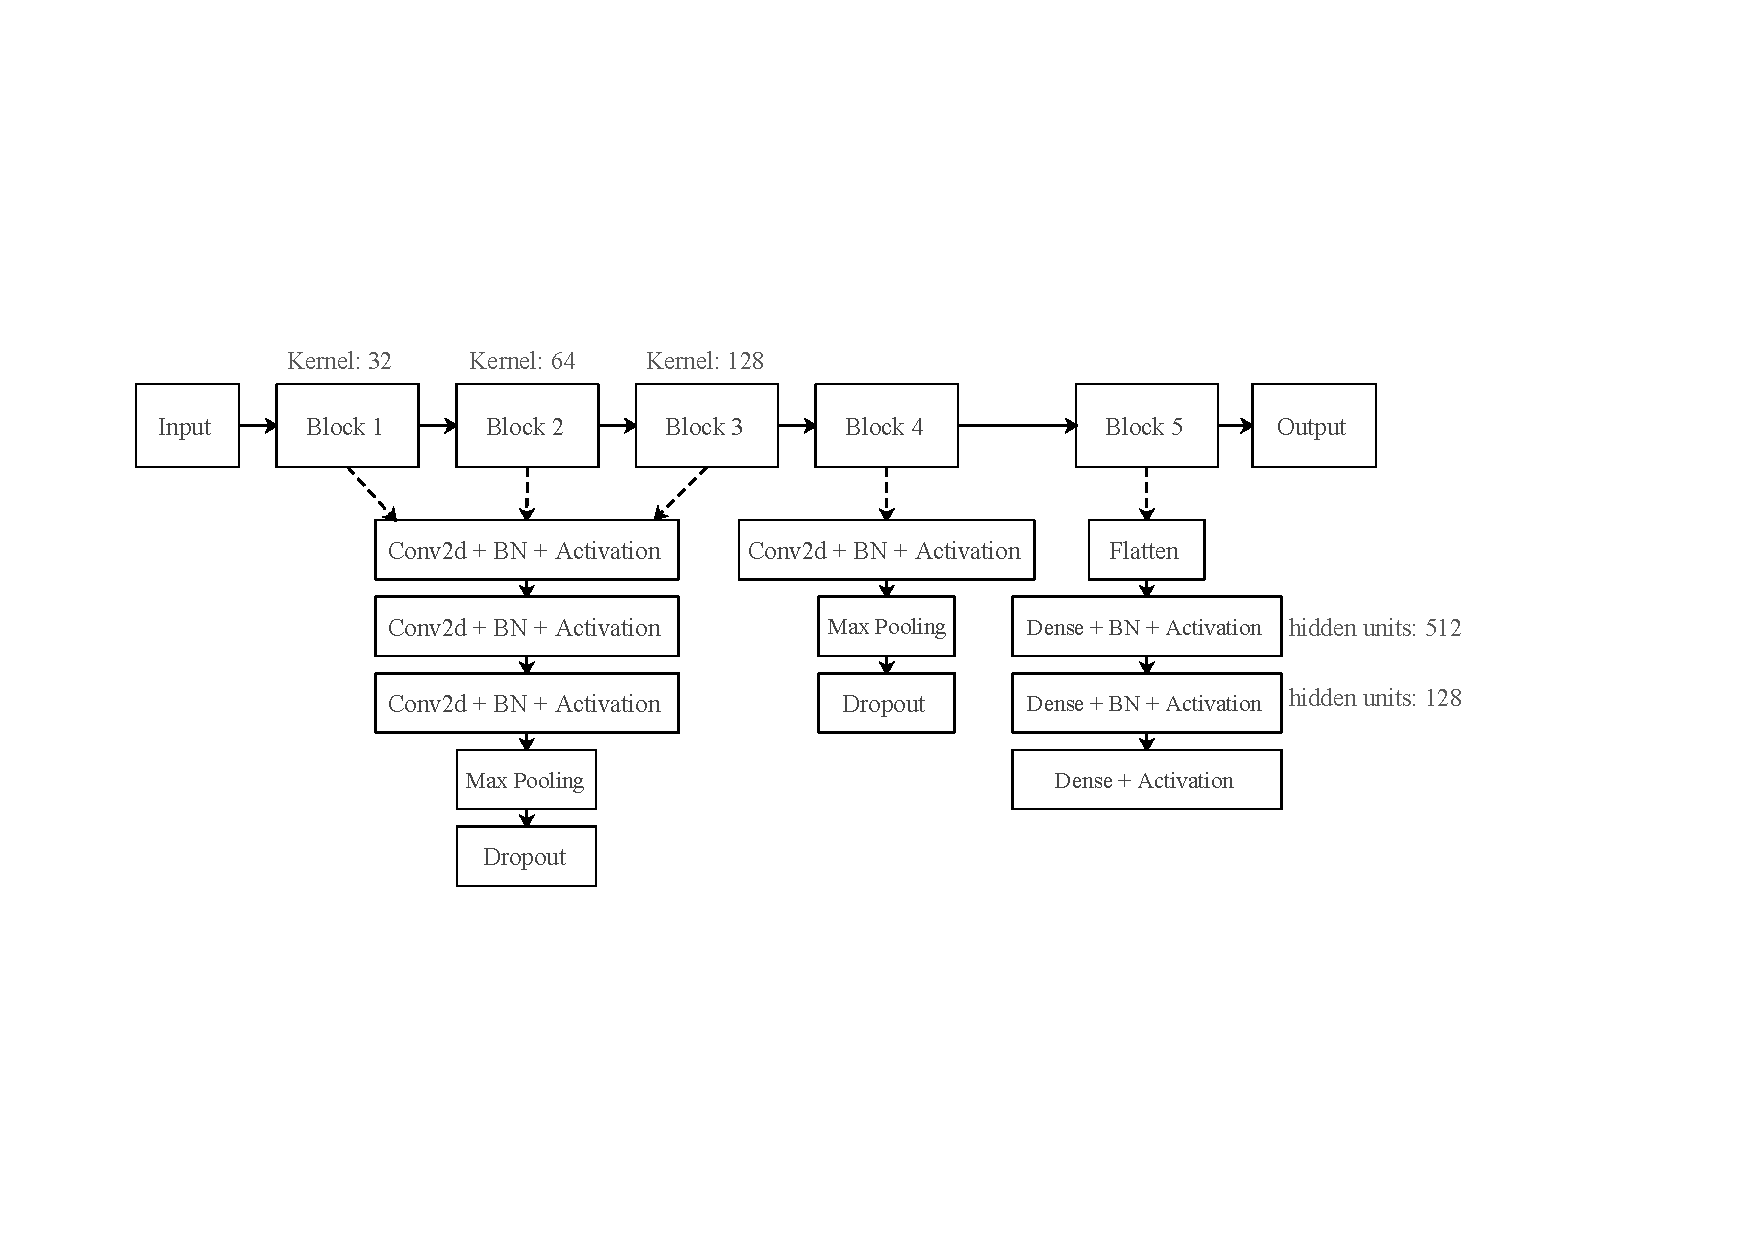
\includegraphics[width=14.5cm]{figs/model}
    \caption{Convolutional neural network}
    \label{fig:modelcnn}
\end{figure}

\paragraph{Implementation}
We implement the CNN model using Keras with TensorFlow as the backend. Our code is available at \url{https://github.com/LuChang-CS/CS583-2019F/tree/master/homework/project/code}. We run the code on a PC with one Intel i9 CPU, 64GB memory and an NVIDIA GeForce RTX 2080Ti GPU. It takes 7 minutes to train the model.

\paragraph{Settings}
The loss function is categorical cross-entropy. The opitmizer is Adam. The batch size is 1024. We use learning decay method, and the initial learning rate is 0.001.

\paragraph{Advanced Tricks}
We applied the following tricks.
\begin{multicols}{3}
\begin{itemize}
    \item Data augmentation
    \item Learning rate decay
    \item Early stopping
    \item Batch normalization
    \item Dropout
\end{itemize}
\end{multicols}

\paragraph{Cross-validation}
We split the training data to 90\%-10\% for hyperparameter tuning. \figurename{~\ref{fig:cnn_result}} plots the convergence curves on 90\% training data and 10\% validation data.
\begin{figure}[H]
    \centering
    \subfloat[][Accuracy]{
        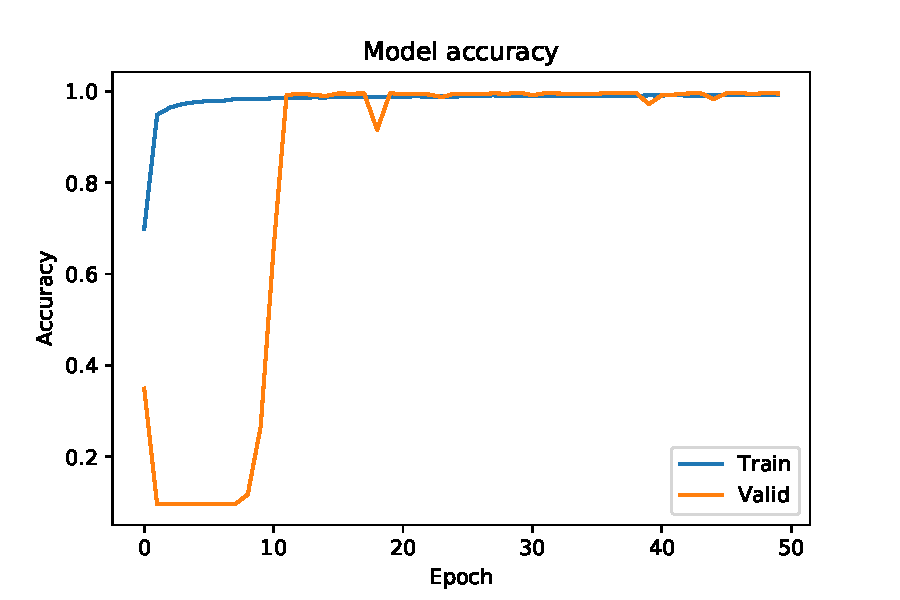
\includegraphics[width=5.5cm]{figs/acc_cnn}
    }
    \subfloat[][Accuracy]{
        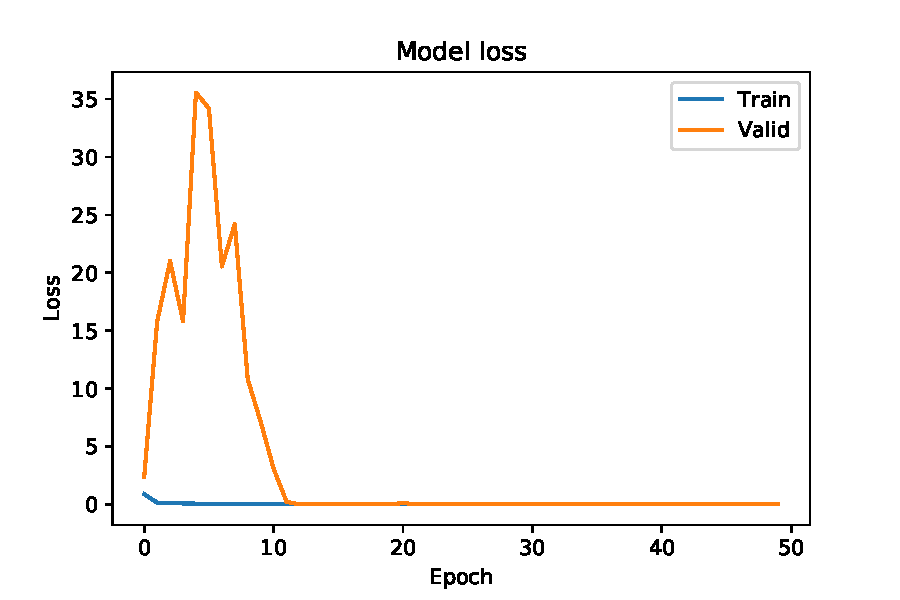
\includegraphics[width=5.5cm]{figs/loss_cnn}
    }
    \caption{Convolutional neural network}
    \label{fig:cnn_result}
\end{figure}

\section{Compared Models}

\paragraph{Convolution Neural Network}
We implement the CNN model as described in the previous section. The training and validation accuracy are 99.21\% and 99.57\% respectively.

\paragraph{Random Guess}
We use a random guess method as the na\"ive baseline. For an input image, it selects a label from 0 to 9 randomly. The training and validation accuracy are 10.13\% and 9.85\% respectively. The public score is 0.09560.

\paragraph{Deep Neural Network}
We implement a 4-hidden-layer deep neural network using Keras. The hidden unit in each layer is 512, 256, 238 and 64. We apply batch normalization in each hidden layer. The training and validation accuracy are 97.12\% and 98.82\% respectively after 50 epochs. The public score is 0.95500.

\section{Outcome}
We participated in an active competition. Our score is 0.98940 in the public leaderboard and the private score will not be available until December 17, 2019. We rank 65/947 in the public leaderboard up to November 30, 2019. The screenshots are in \figurename{~\ref{fig:rank}}.
\begin{figure}[H]
    \centering
    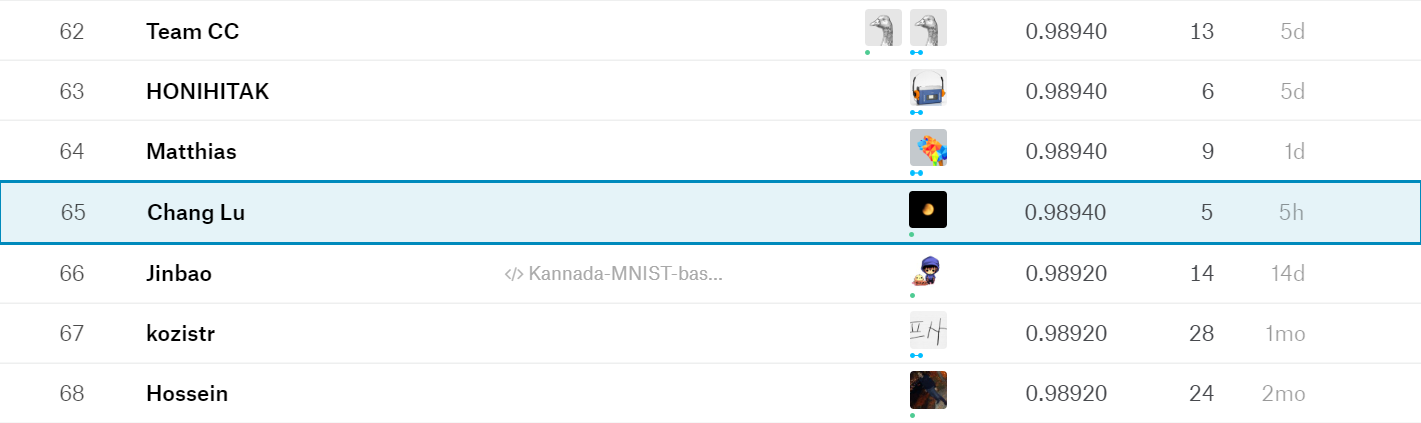
\includegraphics[width=14.5cm]{figs/rank}
    \caption{Our rankings in the leaderboard.}
    \label{fig:rank}
\end{figure}

\printbibliography

\end{document}
